\chapter{جبر خطی و گراف‌ها}
\textbf{یادآوری:}
در این جلسه (جلسه‌ی نهم)، زیر‌فضا‌های بنیادی ماتریس $A$ یادآوری شد، دو مثال از آن در اسلاید‌های ۵ و ۶ حل شد و سپس بخش مربوط به گراف‌ها و شبکه‌ها توضیح داده شد.\\
\textbf{گراف‌ها}

هر گراف با زوج مرتب $(V,E)$ معرفی می‌شود که در آن $V$ مجموعه‌ی رئوس گراف و $E$ مجموعه‌ی یال‌های گراف است. فرض کنید $|V|=n$ و $|E|=m$ باشد. در این صورت ماتریس وقوع یال - رأس $A_{m\times n}$ را به این صورت به آن نسبت می‌دهیم $(A\in M_{mn}(R))$:
اگر یالی از رأس $j$ به رأس $k$ باشد، در سطر متناظر آن یال در ستون $j$ام ۱- گذاشته و در ستون $k$ام ۱+ می‌گذاریم؛ در غیر این صورت، در این درایه‌ها، صفر قرار می‌دهیم.\\
\textbf{مثال:} در زیر، ماتریس $A^T$ مربوط به گراف نمایش داده شده، نوشته شده است:

\begin{center}
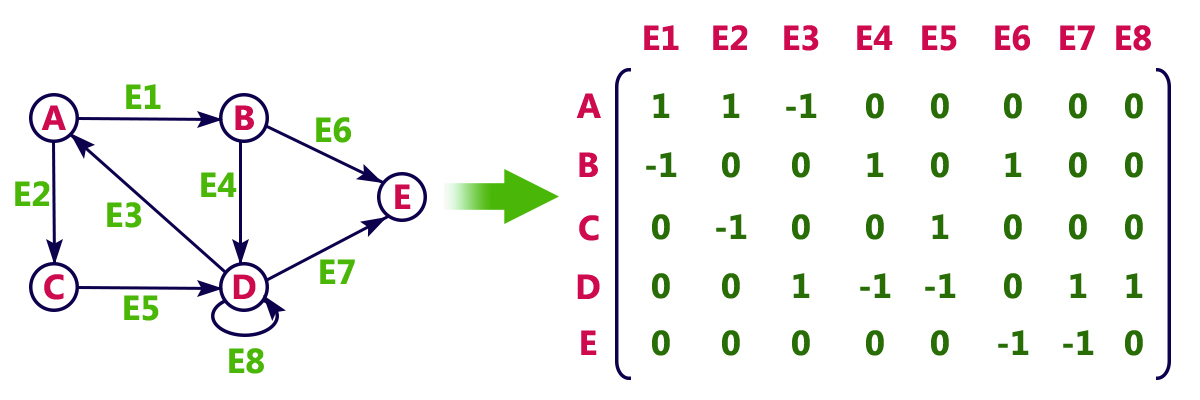
\includegraphics{incidence.jpg}
\end{center}

$A^T$ را ماتریس وقوع رأس - یال می‌نامند.(در نظریه‌ی گراف معمولاً $A^T$ را ماتریس وقوع می‌نامند).\\
حال، چهار زیر‌فضا‌ی بنیادی مربوط به گراف $A$ را بررسی می‌کنیم و معادلی که در گراف دارند را تشریح می‌کنیم. همچنین به اختلاف پتانسیل و شدت جریان در مدار الکتریکی که قابل بازنویسی با یک گراف (جهت‌دار) می‌باشند می‌پردازیم.\\\\
\textbf{فضا‌ی پوچ $A$}\\
در نگاه اول در‌ می‌یابید که حاصل‌جمع ستون‌ها صفر است؛ بنابراین اگر $A_i$ ستون $i$ام $A$ باشد، داریم:
$$A_1+\cdots+A_n= \begin{bmatrix}
A_1 & \cdots & A_n
\end{bmatrix}\begin{bmatrix}
1 \\ \vdots \\ 1
\end{bmatrix}=A\begin{bmatrix}
1 \\ \vdots \\ 1
\end{bmatrix}=0 \quad\Rightarrow\quad \begin{bmatrix}
1 \\ \vdots \\ 1
\end{bmatrix} \in N(A)$$
از طرفی از حل $Ax=0$، با توجه به نحوه‌ی قرارگیری $1$ و $-1$ در سطر اول، به $x_1-x_2=0$ می‌رسیم. اگر $x_2-x_1$ را پتانسیل هر کدام از رئوس فرض کنید، اختلاف پتانسیل دو سر یال ۱ برابر است با $x_2-x_1$. به طور مشابه به ازای هر سطر (که معادل یال است). \\
چون گراف هم‌بند است، پس:
$$x_1=x_2=\cdots=x_n$$ 
بنابراین:
$$x = c\begin{bmatrix}
1 \\ \vdots \\ 1
\end{bmatrix}$$
پس $N(A)$ با بردار $\begin{bmatrix}
1 \\ \vdots \\ 1
\end{bmatrix}$ تولید می‌شود و $dim \: N(A)=1$. بنابر قضیه‌ای که دیدیم :
$$dim\:N(A)+dim\:C(A) = n$$
پس:
$$dim\:C(A)=4-1=3$$
\textbf{فضا‌ی ستونی}\\
دیدیم که $dim \: C(A) = 3$. بنابراین بعد فضا‌ی خطی همه‌ی بردار‌های $b$ که $Ax=b$، برابر با ۳ است. همان‌طور که دیدید از حل $Ax = b$ به معادلات $b_1+b_3=b_2$ و $b_3+b_5=b_4$ می‌رسیم. پس $b$ در فضا‌ی ستونی $A$ است اگر و تنها اگر در معادله‌ی فوق صدق کند.\\
از حل معادله به دست می‌آید که:
$$x_3-x_2=b_3\quad , \quad x_3-x_1= b_2 \quad , \quad x_2-x_1 = b_1$$
$$\underbrace{(x_2-x_1) +(x_3-x_2)=x_3-x_1}_\text{مجموع اختلاف پتانسیل در یک حلقه صفر است.(KVL)} $$
$$b_1+b_3=b_2$$
به طریق مشابه $b_3+b_5=b_4$ که تعبیر آن KVL در حلقه‌ی دوم است.\\\\
\textbf{فضا‌ی پوچ چپ}

از تلاش برای حل معادله‌ی $A^T y = 0$ به‌دست می‌آوریم (راس‌ها و یال‌ها، نام‌گذاری شده‌اند):


\tikzset{every picture/.style={line width=0.75pt}} %set default line width to 0.75pt        

\begin{tikzpicture}[x=0.75pt,y=0.75pt,yscale=-1,xscale=1]
%uncomment if require: \path (0,132); %set diagram left start at 0, and has height of 132

%Shape: Rectangle [id:dp8490539072342648] 
\draw   (68,31) -- (199,31) -- (199,98.25) -- (68,98.25) -- cycle ;
%Straight Lines [id:da3795064505168261] 
\draw    (199,31) -- (68,98.25) ;
\draw   (124,23) -- (139,31.13) -- (124,39.25) ;
\draw   (76,53.25) -- (68.19,67.63) -- (60.38,53.25) ;
\draw   (123,90) -- (138,98.13) -- (123,106.25) ;
\draw   (206,56.25) -- (198.19,70.63) -- (190.38,56.25) ;
\draw   (118.22,80.92) -- (101.86,80.84) -- (110.82,67.15) ;

% Text Node
\draw (128,5) node [anchor=north west][inner sep=0.75pt]   [align=left] {\begin{minipage}[lt]{8.67pt}\setlength\topsep{0pt}
	\begin{flushright}
	۱
	\end{flushright}
	
	\end{minipage}};
% Text Node
\draw (45,54) node [anchor=north west][inner sep=0.75pt]   [align=left] {\begin{minipage}[lt]{8.67pt}\setlength\topsep{0pt}
	\begin{flushright}
	۲
	\end{flushright}
	
	\end{minipage}};
% Text Node
\draw (114,55) node [anchor=north west][inner sep=0.75pt]   [align=left] {\begin{minipage}[lt]{8.67pt}\setlength\topsep{0pt}
	\begin{flushright}
	۳
	\end{flushright}
	
	\end{minipage}};
% Text Node
\draw (212,55) node [anchor=north west][inner sep=0.75pt]   [align=left] {\begin{minipage}[lt]{8.67pt}\setlength\topsep{0pt}
	\begin{flushright}
	۴
	\end{flushright}
	
	\end{minipage}};
% Text Node
\draw (127,111) node [anchor=north west][inner sep=0.75pt]   [align=left] {\begin{minipage}[lt]{8.67pt}\setlength\topsep{0pt}
	\begin{flushright}
	۵
	\end{flushright}
	
	\end{minipage}};
% Text Node
\draw (52,13) node [anchor=north west][inner sep=0.75pt]   [align=left] {\begin{minipage}[lt]{9.530625pt}\setlength\topsep{0pt}
	\begin{flushright}
	A
	\end{flushright}
	
	\end{minipage}};
% Text Node
\draw (202,12) node [anchor=north west][inner sep=0.75pt]   [align=left] {\begin{minipage}[lt]{9.530625pt}\setlength\topsep{0pt}
	\begin{flushright}
	B
	\end{flushright}
	
	\end{minipage}};
% Text Node
\draw (53,101) node [anchor=north west][inner sep=0.75pt]   [align=left] {\begin{minipage}[lt]{10.09375pt}\setlength\topsep{0pt}
	\begin{flushright}
	C
	\end{flushright}
	
	\end{minipage}};
% Text Node
\draw (200,101.25) node [anchor=north west][inner sep=0.75pt]   [align=left] {\begin{minipage}[lt]{10.09375pt}\setlength\topsep{0pt}
	\begin{flushright}
	D
	\end{flushright}
	
	\end{minipage}};


\end{tikzpicture}

راس $A$: $-y_1 -y_2=0$

راس $B$: $y_1 - y_3 - y_4 = 0$

راس $C$: $y_2 + y_3 - y_5 = 0$

راس $D$: $y_4 + y_5 = 0$

اگر $y_i$ ها را جریان عبوری فرض کنیم، معادلات فوق، مجموع جریان هر راس را نشان می‌دهند.

۱- تلاش می‌کنیم برای فضا‌ی خطی $y$هایی که $A^Ty=0$ (معادلاً فضا‌ی پوچ چپ $A$)، یک پایه بیابیم.\\
ابتدا به این سوال پاسخ می‌دهیم که بعد این فضا چیست؟ بعد $A$ برابر با ۳ بود؛ در نتیجه:
$$dim\:N(A^T)=m-r=5-3=2$$
پس بایستی برداری مستقل خطی بیابیم که $A^Ty=0$. از معادلات (*) دریافتیم که جریان در هیچ رأسی ذخیره نمی‌شود و در همه‌ی گراف از جمله داخل حلقه‌های کوچک می‌چرخد. حال به حلقه‌ها نگاه می‌کنیم.

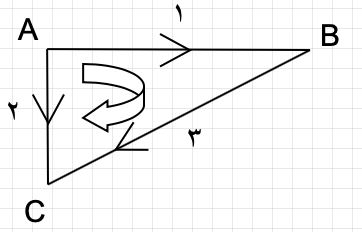
\includegraphics{triangle.png}

$$ y = \begin{bmatrix}
1 \\ -1 \\ 1 \\ 0 \\ 0
\end{bmatrix} $$

$$ \begin{bmatrix}
-1 & -1 & 0 & 0 & 0 \\
1 & 0 & -1 & -1 & 0 \\
0 & 1 & 1 & 0 & -1 \\
0 & 0 & 0 & 1 & 1
\end{bmatrix} 
\begin{bmatrix}
1 \\ -1 \\ 1 \\ 0 \\ 0
\end{bmatrix}
=
\begin{bmatrix}
-1+1 \\ 1+0-1 \\ -1+1+0 \\ 0
\end{bmatrix}
=
\begin{bmatrix}
0 \\ 0 \\ 0 \\ 0
\end{bmatrix}
$$


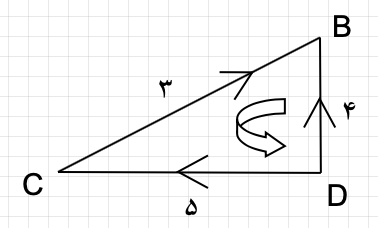
\includegraphics{triangle2.png}

$$
y = \begin{bmatrix}
0 \\ 0 \\ 1 \\ -1 \\ 1
\end{bmatrix} 
$$

$$ A^T y' = 0 $$

در نتیجه، دو بردار فوق در $N(A^T)$ قرار داشته، مستقل خطی بوده و $dim(N(A^T)) = 2$، پس پایه‌ای برای $N(A^T)$ هستند. در غیاب جریان‌های منبع، هر بردار در $N(A^T)$ نشان‌گر یک بردار جریان در مدار است که در حال چرخش است، یعنی KCL (مجموع جریان‌ها در هر راس صفر است).
حال اگر در رئوسی از مدار، مشابه مثال مدار ارائه شده، منبع جریان داشته باشیم، برای محاسبه‌ی جریان، باید به محاسبه‌ی $A^Ty=f$ بپردازیم که در حضور منابعی از جریان $A^Ty=f$ در رأس‌ها متناظر قانون KCL است که کل جریان ورودی برابر با جریان خروجی است. \\
بنابراین فضا‌های بنیادی منسوب به $A$ را مطالعه کردیم. حال فرض کنید مدار داده شده است (مشابه اسلاید‌ها)؛ می‌توان برای محاسبه‌ی $y$ (جریان‌ها) از معادله‌ی $A^T=f$ و برای محاسبه‌ی پتانسیل‌ها از $A^TcAx=A^Tcb-f$، مطابق محاسبات انجام شده در اسلاید‌ها، ‌استفاده کرد.

